% Toolbar icon: edgeLength — a curved edge with endpoint dots over a dimension bracket;
% the curve is what distinguishes it from distance.tex's straight measurement.
\documentclass[tikz,border=2mm]{standalone}
\usetikzlibrary{arrows.meta,calc,shapes.geometric}
\begin{document}
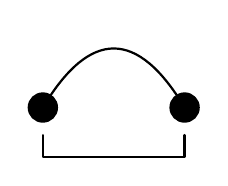
\begin{tikzpicture}[line width=1.3pt, line cap=round, line join=round, >=Stealth, x=1mm,y=1mm]
  \draw[thick] (-9,-3.5) .. controls (-3,6.5) and (3,6.5) .. (9,-3.5);
  \filldraw (-9,-3.5) circle (1.7);
  \filldraw (9,-3.5) circle (1.7);
  \draw[thick] (-9,-7) -- (-9,-9.8) -- (9,-9.8) -- (9,-7);
\end{tikzpicture}
\end{document}
